\documentclass[
	10pt,
	a4j,		% 余白小
%	a4paper,	% 余白普通
	twocolumn,	% 二段組
	uplatex
]{jsarticle}

\usepackage{iml_redume}


%% コマンドの置き換え(お好みで)
\usepackage{letltxmacro}	% 安全にコマンドを置き換える
\AtBeginDocument{
	% 賢いrefに置き換え
	\LetLtxMacro{\oldref}{\ref}
	\renewcommand{\ref}{\cref}
}


% ヘッダーの設定
\lhead{\small\textbf{2017年度 卒業論文発表会(2018年1月1日)}}
\rhead{\small\textbf{知的機構研究室}}
\cfoot{}	% ページ番号なし

\title{ぞうの卵のぞうの卵によるぞうの卵ためのぞうの卵 \linebreak 象卵の象卵による象卵ための象卵}
\author{姓 名}

\begin{document}
\maketitle

\section{はじめに}
\label{sec:introduction}
ぞうの卵はおいしいぞう\footnote{あくまで個人の感想です.}.ぞうの卵はおいしいぞう.ぞうの卵はおいしいぞう.ぞうの卵はおいしいぞう.ぞうの卵はおいしいぞう.ぞうの卵はおいしいぞう.ぞうの卵はおいしいぞう.ぞうの卵はおいしいぞう.ぞうの卵はおいしいぞう.ぞうの卵はおいしいぞう.ぞうの卵はおいしいぞう.ぞうの卵はおいしいぞう.ぞうの卵はおいしいぞう.ぞうの卵はおいしいぞう.ぞうの卵はおいしいぞう.ぞうの卵はおいしいぞう.ぞうの卵はおいしいぞう.ぞうの卵はおいしいぞう.ぞうの卵はおいしいぞう.ぞうの卵はおいしいぞう.ぞうの卵はおいしいぞう.ぞうの卵はおいしいぞう.ぞうの卵はおいしいぞう.ぞうの卵はおいしいぞう.ぞうの卵はおいしいぞう.ぞうの卵はおいしいぞう.ぞうの卵はおいしいぞう.ぞうの卵はおいしいぞう.ぞうの卵はおいしいぞう.ぞうの卵はおいしいぞう.ぞうの卵はおいしいぞう.ぞうの卵はおいしいぞう.ぞうの卵はおいしいぞう.ぞうの卵はおいしいぞう.ぞうの卵はおいしいぞう.ぞうの卵はおいしいぞう.ぞうの卵はおいしいぞう.ぞうの卵はおいしいぞう.ぞうの卵はおいしいぞう.ぞうの卵はおいしいぞう.ぞうの卵はおいしいぞう.ぞうの卵はおいしいぞう.ぞうの卵はおいしいぞう.ぞうの卵はおいしいぞう.ぞうの卵はおいしいぞう.ぞうの卵はおいしいぞう.ぞうの卵はおいしいぞう.ぞうの卵はおいしいぞう.ぞうの卵はおいしいぞう.ぞうの卵はおいしいぞう.ぞうの卵はおいしいぞう.ぞうの卵はおいしいぞう.ぞうの卵はおいしいぞう.ぞうの卵はおいしいぞう.ぞうの卵はおいしいぞう.ぞうの卵はおいしいぞう.ぞうの卵はおいしいぞう.ぞうの卵はおいしいぞう.ぞうの卵はおいしいぞう.ぞうの卵はおいしいぞう.ぞうの卵はおいしいぞう.ぞうの卵はおいしいぞう.ぞうの卵はおいしいぞう.ぞうの卵はおいしいぞう.ぞうの卵はおいしいぞう.ぞうの卵はおいしいぞう.ぞうの卵はおいしいぞう.ぞうの卵はおいしいぞう.

\subsection{そして}
ぞうの卵はおいしいぞう.ぞうの卵はおいしいぞう.ぞうの卵はおいしいぞう.ぞうの卵はおいしいぞう.ぞうの卵はおいしいぞう.ぞうの卵はおいしいぞう.ぞうの卵はおいしいぞう.ぞうの卵はおいしいぞう.ぞうの卵はおいしいぞう.ぞうの卵はおいしいぞう.ぞうの卵はおいしいぞう.ぞうの卵はおいしいぞう.ぞうの卵はおいしいぞう.ぞうの卵はおいしいぞう.ぞうの卵はおいしいぞう.ぞうの卵はおいしいぞう.ぞうの卵はおいしいぞう.ぞうの卵はおいしいぞう.ぞうの卵はおいしいぞう.ぞうの卵はおいしいぞう.ぞうの卵はおいしいぞう.ぞうの卵はおいしいぞう.ぞうの卵はおいしいぞう.ぞうの卵はおいしいぞう.ぞうの卵はおいしいぞう.ぞうの卵はおいしいぞう.ぞうの卵はおいしいぞう.ぞうの卵はおいしいぞう.ぞうの卵はおいしいぞう.ぞうの卵はおいしいぞう.ぞうの卵はおいしいぞう.ぞうの卵はおいしいぞう.ぞうの卵はおいしいぞう.ぞうの卵はおいしいぞう.ぞうの卵はおいしいぞう.ぞうの卵はおいしいぞう.ぞうの卵はおいしいぞう.ぞうの卵はおいしいぞう.ぞうの卵はおいしいぞう.ぞうの卵はおいしいぞう.ぞうの卵はおいしいぞう.ぞうの卵はおいしいぞう.ぞうの卵はおいしいぞう\cite{110001167075,120002205324,mr1763essay,fisher1925statistical}.


\begin{figure}[t]
	\centering
	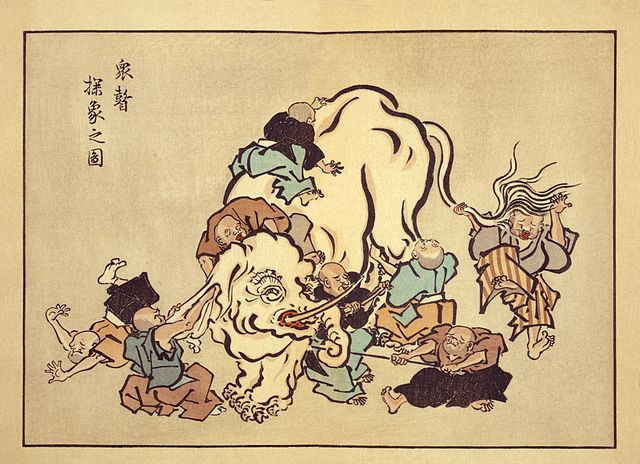
\includegraphics[clip,width=0.5\textwidth]{fig/elephant.jpg}
	\caption{
		群盲象を評す.
		\label{fig:elephant}
	}
\end{figure}

ぞうの卵はおいしいぞう.ぞうの卵はおいしいぞう.ぞうの卵はおいしいぞう.ぞうの卵はおいしいぞう.ぞうの卵はおいしいぞう.ぞうの卵はおいしいぞう.ぞうの卵はおいしいぞう.ぞうの卵はおいしいぞう.ぞうの卵はおいしいぞう.ぞうの卵はおいしいぞう.ぞうの卵はおいしいぞう.ぞうの卵はおいしいぞう.ぞうの卵はおいしいぞう.ぞうの卵はおいしいぞう.ぞうの卵はおいしいぞう.ぞうの卵はおいしいぞう.ぞうの卵はおいしいぞう.ぞうの卵はおいしいぞう.ぞうの卵はおいしいぞう.ぞうの卵はおいしいぞう.ぞうの卵はおいしいぞう.ぞうの卵はおいしいぞう.ぞうの卵はおいしいぞう(\ref{fig:elephant}).

\subparagraph{手法1}
ぞうの卵はおいしいぞう.ぞうの卵はおいしいぞう.ぞうの卵はおいしいぞう.ぞうの卵はおいしいぞう.ぞうの卵はおいしいぞう.ぞうの卵はおいしいぞう.ぞうの卵はおいしいぞう.ぞうの卵はおいしいぞう.ぞうの卵はおいしいぞう.ぞうの卵はおいしいぞう.ぞうの卵はおいしいぞう.ぞうの卵はおいしいぞう.ぞうの卵はおいしいぞう.ぞうの卵はおいしいぞう.ぞうの卵はおいしいぞう.ぞうの卵はおいしいぞう.ぞうの卵はおいしいぞう.ぞうの卵はおいしいぞう.ぞうの卵はおいしいぞう.ぞうの卵はおいしいぞう.

\subparagraph{手法2}
ぞうの卵はおいしいぞう.ぞうの卵はおいしいぞう.ぞうの卵はおいしいぞう.ぞうの卵はおいしいぞう.ぞうの卵はおいしいぞう.ぞうの卵はおいしいぞう.ぞうの卵はおいしいぞう.ぞうの卵はおいしいぞう.ぞうの卵はおいしいぞう.ぞうの卵はおいしいぞう.ぞうの卵はおいしいぞう.ぞうの卵はおいしいぞう.ぞうの卵はおいしいぞう.ぞうの卵はおいしいぞう.

\begin{itemize}
	\item ぞうの卵はおいしいぞう.
	\item ぞうの卵はおいしいぞう.
	\item ぞうの卵はおいしいぞう.
\end{itemize}
\begin{enumerate}
	\item ぞうの卵はおいしいぞう.
	\item ぞうの卵はおいしいぞう.
	\item ぞうの卵はおいしいぞう.
\end{enumerate}

\begin{figure}[t]
	\centering
	
\includegraphics[clip,width=0.5\textwidth]{fig/LaTeX.pdf}
	\caption{
		\LaTeX{}の図.
		\label{fig:latex}
	}
\end{figure}

\section{つぎに}
\begin{table}[t]
	\centering
	\caption{
		価格表.
		\label{tab:egg}
	}
	\begin{tabular}{l|cr}
		\toprule
		名称    &   数量  &   金額 \\
		\midrule
		ネズミの卵   &   1    &   1,000 \\
		ゾウの卵   &   2    &   3,000 \\
		ごまたまご &	12 & 1,000 \\
		\bottomrule
	\end{tabular}
\end{table}

\ref{sec:introduction}でも述べたようにゾウの卵はおいしいぞう(\ref{tab:egg}).ゾウの卵はおいしいぞう.ゾウの卵はおいしいぞう.ゾウの卵はおいしいぞう.ゾウの卵はおいしいぞう.ゾウの卵はおいしいぞう.ゾウの卵はおいしいぞう.ゾウの卵はおいしいぞう.ゾウの卵はおいしいぞう.ゾウの卵はおいしいぞう.ゾウの卵はおいしいぞう.ゾウの卵はおいしいぞう.ゾウの卵はおいしいぞう.ゾウの卵はおいしいぞう.ゾウの卵はおいしいぞう.ゾウの卵はおいしいぞう.ゾウの卵はおいしいぞう.ゾウの卵はおいしいぞう.ゾウの卵はおいしいぞう.ゾウの卵はおいしいぞう.ゾウの卵はおいしいぞう.ゾウの卵はおいしいぞう.ゾウの卵はおいしいぞう.ゾウの卵はおいしいぞう.ゾウの卵はおいしいぞう.ゾウの卵はおいしいぞう.ゾウの卵はおいしいぞう.ゾウの卵はおいしいぞう.ゾウの卵はおいしいぞう.ゾウの卵はおいしいぞう.ゾウの卵はおいしいぞう.ゾウの卵はおいしいぞう.ゾウの卵はおいしいぞう.ゾウの卵はおいしいぞう.ゾウの卵はおいしいぞう.ゾウの卵はおいしいぞう.ゾウの卵はおいしいぞう.ゾウの卵はおいしいぞう.ゾウの卵はおいしいぞう.ゾウの卵はおいしいぞう.ゾウの卵はおいしいぞう.ゾウの卵はおいしいぞう.ゾウの卵はおいしいぞう.ゾウの卵はおいしいぞう.ゾウの卵はおいしいぞう.ゾウの卵はおいしいぞう.ゾウの卵はおいしいぞう.ゾウの卵はおいしいぞう.ゾウの卵はおいしいぞう.ゾウの卵はおいしいぞう.ゾウの卵はおいしいぞう.ゾウの卵はおいしいぞう.ゾウの卵はおいしいぞう.ゾウの卵はおいしいぞう.ゾウの卵はおいしいぞう.ゾウの卵はおいしいぞう.ゾウの卵はおいしいぞう.ゾウの卵はおいしいぞう.ゾウの卵はおいしいぞう.ゾウの卵はおいしいぞう.ゾウの卵はおいしいぞう.ゾウの卵はおいしいぞう.ゾウの卵はおいしいぞう.ゾウの卵はおいしいぞう.ゾウの卵はおいしいぞう.ゾウの卵はおいしいぞう.ゾウの卵はおいしいぞう.ゾウの卵はおいしいぞう.ゾウの卵はおいしいぞう.ゾウの卵はおいしいぞう.ゾウの卵はおいしいぞう.ゾウの卵はおいしいぞう.ゾウの卵はおいしいぞう.ゾウの卵はおいしいぞう.ゾウの卵はおいしいぞう.ゾウの卵はおいしいぞう.

\begin{align}
a &= b	\\
&= c	\notag\\
&= d.
\end{align}

\begin{equation}
\begin{aligned}
a &= b	\\
&= c	\\
&= d.
\end{aligned}
\label{eq:equation}
\end{equation}

\begin{equation}
|a| =
\begin{cases}
a  & \text{if $a>0$,}\\
-a & \text{if $a<0$.}
\end{cases}
\end{equation}

\ref{eq:equation}は自明.This document contains English, Română, Español and 日本語. This document contains English, Română, Español and 日本語. This document contains English, Română, Español and 日本語. This document contains English, Română, Español and 日本語. This document contains English, Română, Español and 日本語. This document contains English, Română, Español and 日本語. This document contains English, Română, Español and 日本語. This document contains English, Română, Español and 日本語. This document contains English, Română, Español and 日本語. This document contains English, Română, Español and 日本語. This document contains English, Română, Español and 日本語. This document contains English, Română, Español and 日本語. This document contains English, Română, Español and 日本語. 

\begin{algorithm}[t]
	\caption{Calculate $y = x^n$}
	\label{alg:algorithm}
	\begin{algorithmic}[1]
		\Require	$n \geq 0 \vee x \neq 0$
		\Ensure	$y = x^n$
		\State $y \Leftarrow 1$
			\If{$n < 0$}
				\State $X \Leftarrow 1 / x$
				\State $N \Leftarrow -n$
			\Else
				\State $X \Leftarrow x$
				\State $N \Leftarrow n$
			\EndIf
		\While{$N \neq 0$}
			\If{$N$ is even}
				\State $X \Leftarrow X \times X$
				\State $N \Leftarrow N / 2$
			\Else[$N$ is odd]
				\State $y \Leftarrow y \times X$
				\State $N \Leftarrow N - 1$
			\EndIf
		\EndWhile
	\end{algorithmic}
\end{algorithm}

{\footnotesize
	%% 参考文献
	\bibliographystyle{ipsjunsrt}
	\bibliography{sample_ref}
	
	%% 業績 なければコメントアウト
	% 丸括弧にする
	\makeatletter
	\renewcommand{\@biblabel}[1]{#1)}
	\makeatother
	\bibliographystyleachieve{ipsjunsrt}
	\bibliographyachieve{achievement}
	\nociteachieve{*}
}

\end{document}